\documentclass[11pt,letterpaper]{article}
\usepackage[utf8]{inputenc}

%----- Configuración del estilo del documento------%
\usepackage[table]{xcolor}
\usepackage{epsfig,graphicx}
\usepackage[left=2cm,right=2cm,top=1.8cm,bottom=2.3cm]{geometry}
\usepackage{fancyhdr}
\usepackage{lastpage}
\pagestyle{fancy}
\fancyhf{}
\rfoot{\textit{Página \thepage \hspace{1pt} de \pageref{LastPage}}}


%------ Paquetes matemáticos básicos --------%
\usepackage{amsmath}
\usepackage{amsfonts}
\usepackage{amssymb}
\usepackage{amsthm}
\usepackage{geometry}
\geometry{margin=1in}

%------ Texto aleatorio ----- %

\usepackage{lipsum}
\usepackage{enumitem}


\begin{document}

%------ Encabezado -------- %

\begin{center}
    \begin{minipage}{3cm}
    	\begin{center}
    		\includegraphics[height=3.4cm]{./imagenes/logo_unam.png}
    	\end{center}
    \end{minipage}\hfill
    \begin{minipage}{10cm}
    	\begin{center}
    	\textbf{\large Universidad Nacional Autónoma de México}\\[0.1cm]
        \textbf{Facultad de Ciencias}\\[0.1cm]
        \textbf{Matemáticas para las Ciencias Aplicadas $|$ Grupo 7048}\\[0.1cm]
        \textbf{Tarea 4 }\\[0.1cm]
        Real Araiza Yamile\\[0.1cm]
        Rodríguez López Luis Fernando\\[0.1cm]
        Tenorio Reyes Ihebel Luro\\[0.1cm]
        25/11/2024
    	\end{center}
    \end{minipage}\hfill
    \begin{minipage}{3cm}
    	\begin{center}
    		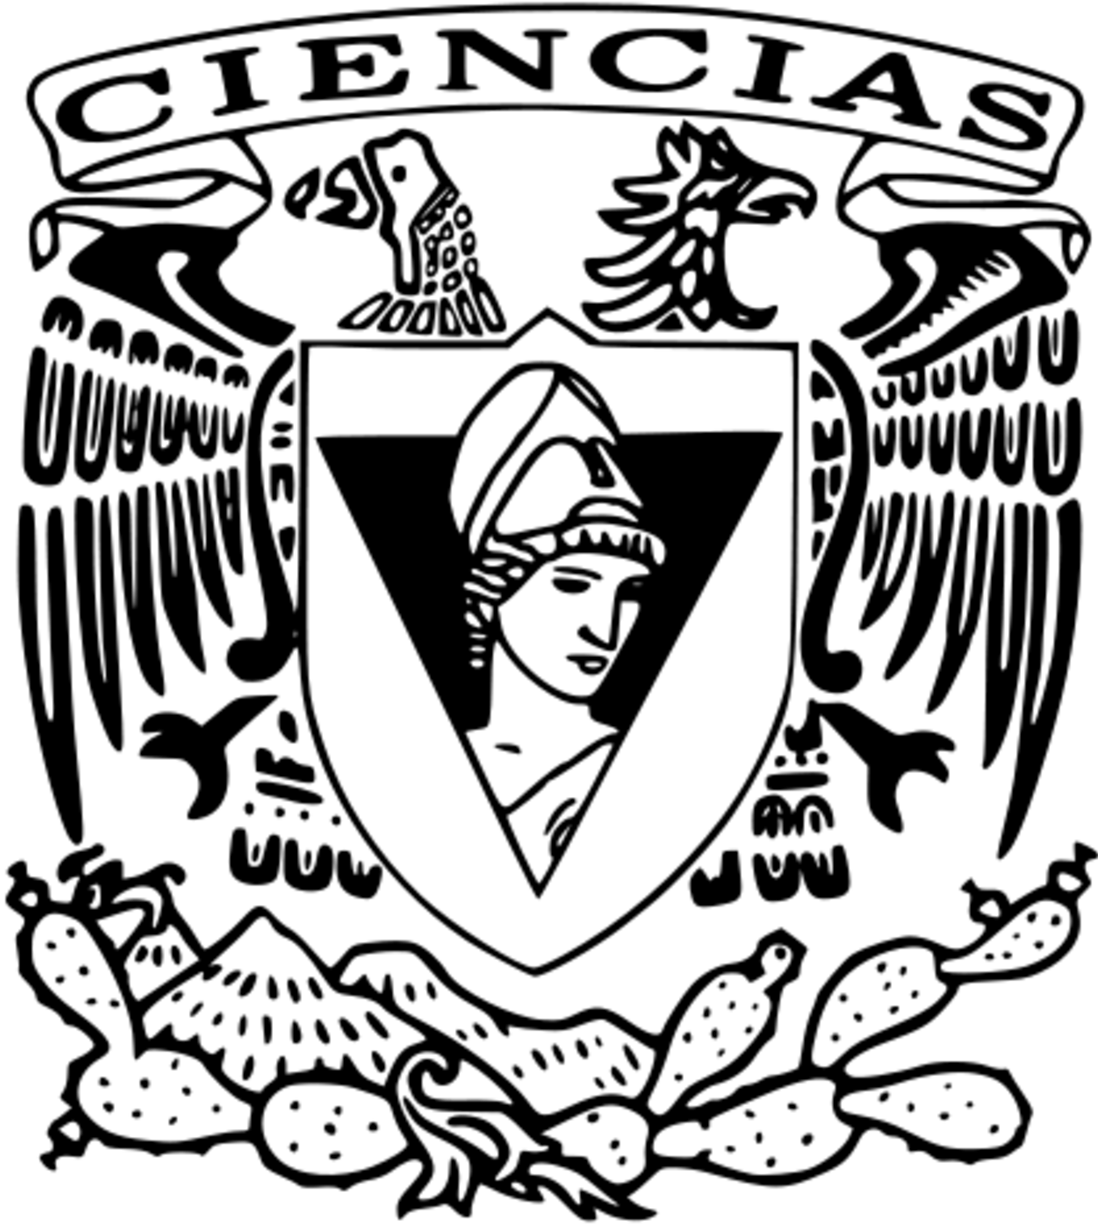
\includegraphics[height=3.4cm]{./imagenes/Logo_FC.png}
    	\end{center}
    \end{minipage}
\end{center}

\rule{17cm}{0.1mm}

%------ Fin de encabezado -------- %

%\section*{1ra Parte}

\subparagraph{Ejercicios: Review Exercises Capítulo 5 Anton-Bivens-Davis (pp. 408-412).}

% ---- 01. Ejercicio 13 IHEBEL ---- %
\section{Ejercicio 13, cap V Review Exercises.}

% ---- 02. Ejercicio 23 YAMILE ---- %
\section{Ejercicio 23, cap V Review Exercises.}
\section*{Cálculo de aproximaciones al área bajo la curva \(y = \ln(x)\)}

Queremos calcular las aproximaciones con los puntos extremos izquierdo, derecho y puntos medios para estimar el área bajo la curva \(y = \ln(x)\) en el intervalo \([1, 2]\) utilizando \(n = 10\) subintervalos.

\subsection*{Paso 1: Determinar el ancho de los subintervalos}
\[
\Delta x = \frac{b - a}{n} = \frac{2 - 1}{10} = 0.1
\]

\subsection*{Paso 2: Determinar los puntos de los subintervalos}
Los puntos que dividen el intervalo \([1, 2]\) en 10 subintervalos son:
\[
x_0 = 1, \, x_1 = 1.1, \, x_2 = 1.2, \dots, x_{10} = 2
\]

\subsection*{Paso 3: Aproximaciones}

\subsubsection*{(a) Aproximación con puntos extremos izquierdos}
Usamos los puntos \(x_0, x_1, \dots, x_9\). La fórmula es:
\[
A_{\text{izq}} = \Delta x \sum_{i=0}^{n-1} f(x_i)
\]
Sustituyendo:
\[
A_{\text{izq}} = 0.1 \left[ \ln(1) + \ln(1.1) + \ln(1.2) + \cdots + \ln(1.9) \right]
\]
Evaluando \(f(x_i) = \ln(x_i)\):
\[
f(x_0) = \ln(1) = 0, \quad f(x_1) = \ln(1.1) \approx 0.0953, \quad f(x_2) = \ln(1.2) \approx 0.1823, \dots, f(x_9) = \ln(1.9) \approx 0.6419
\]
Sumamos los valores:
\[
\sum f(x_i) = 0 + 0.0953 + 0.1823 + 0.2624 + 0.3365 + 0.4055 + 0.4700 + 0.5306 + 0.5878 + 0.6419 = 3.5122
\]
Entonces:
\[
A_{\text{izq}} = 0.1 \cdot 3.5122 = 0.3512
\]

\subsubsection*{(b) Aproximación con puntos extremos derechos}
Usamos los puntos \(x_1, x_2, \dots, x_{10}\). La fórmula es:
\[
A_{\text{der}} = \Delta x \sum_{i=1}^{n} f(x_i)
\]
Sustituyendo:
\[
A_{\text{der}} = 0.1 \left[ \ln(1.1) + \ln(1.2) + \ln(1.3) + \cdots + \ln(2) \right]
\]
Evaluando \(f(x_i) = \ln(x_i)\):
\[
f(x_1) = \ln(1.1) \approx 0.0953, \quad f(x_2) = \ln(1.2) \approx 0.1823, \, \dots, \, f(x_{10}) = \ln(2) \approx 0.6931
\]
Sumamos los valores:
\[
\sum f(x_i) = 0.0953 + 0.1823 + 0.2624 + 0.3365 + 0.4055 + 0.4700 + 0.5306 + 0.5878 + 0.6419 + 0.6931 = 4.2054
\]
Entonces:
\[
A_{\text{der}} = 0.1 \cdot 4.2054 = 0.4205
\]

\subsubsection*{(c) Aproximación con puntos medios}
Usamos los puntos medios de cada subintervalo. La fórmula es:
\[
A_{\text{medio}} = \Delta x \sum_{i=1}^{n} f\left(\frac{x_{i-1} + x_i}{2}\right)
\]
Cálculo de los puntos medios:
\[
x_{\text{medio},1} = \frac{1 + 1.1}{2} = 1.05, \, x_{\text{medio},2} = \frac{1.1 + 1.2}{2} = 1.15, \dots, x_{\text{medio},10} = \frac{1.9 + 2}{2} = 1.95
\]
Evaluando \(f(x)\) en estos puntos medios:
\[
f(1.05) \approx 0.0488, \, f(1.15) \approx 0.1398, \dots, f(1.95) \approx 0.6678
\]
Sumamos los valores:
\[
\sum f(x_{\text{medio}}) = 0.0488 + 0.1398 + 0.2231 + 0.3001 + 0.3716 + 0.4383 + 0.5008 + 0.5593 + 0.6145 + 0.6678 = 3.8650
\]
Entonces:
\[
A_{\text{medio}} = 0.1 \cdot 3.8650 = 0.3865
\]

\subsection*{Resumen de Resultados}
\[
A_{\text{izq}} = 0.3512, \quad A_{\text{der}} = 0.4205, \quad A_{\text{medio}} = 0.3865
\]


% ---- 03. Ejercicio 42 YAMILE ---- %
\section{Ejercicio 42, cap V Review Exercises.}
\section*{Cálculo del área bajo la curva}

Queremos calcular el área bajo la curva \(f(x) = \frac{1}{x}\) en el intervalo \([1, e^3]\). Esto se realiza resolviendo la integral definida:

\[
\int_{1}^{e^3} \frac{1}{x} \, dx
\]

\subsection*{Paso 1: Resolver la integral indefinida}
Sabemos que:
\[
\int \frac{1}{x} \, dx = \ln|x| + C
\]

Por lo tanto, la integral definida es:
\[
\int_{1}^{e^3} \frac{1}{x} \, dx = \ln(x) \Big|_{1}^{e^3}
\]

\subsection*{Paso 2: Evaluar los límites}
Evaluamos los límites de integración:
\[
\ln(e^3) - \ln(1)
\]

Sabemos que:
\[
\ln(e^3) = 3 \quad \text{y} \quad \ln(1) = 0
\]

Por lo tanto:
\[
\ln(e^3) - \ln(1) = 3 - 0 = 3
\]

\subsection*{Resultado final}
El área bajo la curva \(f(x) = \frac{1}{x}\) en el intervalo \([1, e^3]\) es:
\[
\boxed{3}
\]


% ---- 04. Ejercicio 53 LUIS ---- %
\section{Ejercicio 53, cap V Review Exercises.}

% ---- 05. Ejercicio 56 LUIS ---- %
\section{Ejercicio 56, cap V Review Exercises.}

% ---- 06. Ejercicio 64 LUIS ---- %
\section{Ejercicio 64, cap V Review Exercises.}

% ---- 07. Ejercicio 68 IHEBEL ---- %
\section{Ejercicio 68, cap V Review Exercises.}

% ---- 08. Ejercicio 73 LUIS ---- %
\section{Ejercicio 73, cap V Review Exercises.}

% ---- 09. Ejercicio 76 YAMILE ---- %
\section{Ejercicio 76, cap V Review Exercises.}
\section*{Cálculo del desplazamiento y la distancia total recorrida}

Dada la aceleración \(a(t) = \frac{1}{\sqrt{5t + 1}}\) m/s\(^2\) y la velocidad inicial \(v_0 = 2\) m/s, queremos calcular el desplazamiento y la distancia total recorrida por la partícula en el intervalo \(0 \leq t \leq 3\).

\subsection*{Paso 1: Encontrar la velocidad \(v(t)\)}

Sabemos que:
\[
a(t) = \frac{dv}{dt}.
\]

Por lo tanto, la velocidad se obtiene integrando \(a(t)\):
\[
v(t) = \int a(t) \, dt = \int \frac{1}{\sqrt{5t + 1}} \, dt.
\]

Para resolver la integral, usamos el cambio de variable:
\[
u = 5t + 1 \quad \Rightarrow \quad du = 5 \, dt \quad \Rightarrow \quad dt = \frac{du}{5}.
\]

La integral se convierte en:
\[
\int \frac{1}{\sqrt{5t + 1}} \, dt = \int \frac{1}{\sqrt{u}} \cdot \frac{1}{5} \, du = \frac{1}{5} \int u^{-1/2} \, du = \frac{1}{5} \cdot 2u^{1/2} + C.
\]

Sustituyendo \(u = 5t + 1\), obtenemos:
\[
v(t) = \frac{2}{5} \sqrt{5t + 1} + C.
\]

Usamos la condición inicial \(v(0) = 2\) para calcular \(C\):
\[
v(0) = \frac{2}{5} \sqrt{5(0) + 1} + C = 2 \quad \Rightarrow \quad \frac{2}{5}(1) + C = 2 \quad \Rightarrow \quad C = \frac{8}{5}.
\]

Por lo tanto, la expresión para la velocidad es:
\[
v(t) = \frac{2}{5} \sqrt{5t + 1} + \frac{8}{5}.
\]

\subsection*{Paso 2: Calcular el desplazamiento}

El desplazamiento se obtiene integrando \(v(t)\) en el intervalo \(0 \leq t \leq 3\):
\[
\text{Desplazamiento} = \int_{0}^{3} v(t) \, dt = \int_{0}^{3} \left( \frac{2}{5} \sqrt{5t + 1} + \frac{8}{5} \right) \, dt.
\]

Separamos en dos integrales:
\[
\int_{0}^{3} v(t) \, dt = \frac{2}{5} \int_{0}^{3} \sqrt{5t + 1} \, dt + \frac{8}{5} \int_{0}^{3} 1 \, dt.
\]

\subsubsection*{Primera integral}
Usamos nuevamente el cambio de variable \(u = 5t + 1\), con \(du = 5 \, dt\) y \(dt = \frac{du}{5}\). Los límites de integración cambian:
\[
t = 0 \Rightarrow u = 1, \quad t = 3 \Rightarrow u = 16.
\]

La integral se convierte en:
\[
\int_{0}^{3} \sqrt{5t + 1} \, dt = \int_{1}^{16} \sqrt{u} \cdot \frac{1}{5} \, du = \frac{1}{5} \int_{1}^{16} u^{1/2} \, du = \frac{1}{5} \cdot \frac{2}{3} \left[ u^{3/2} \right]_{1}^{16}.
\]

Evaluamos:
\[
\int_{0}^{3} \sqrt{5t + 1} \, dt = \frac{2}{15} \left[ (16)^{3/2} - (1)^{3/2} \right] = \frac{2}{15} \left[ 64 - 1 \right] = \frac{2}{15} \cdot 63 = \frac{126}{15} = 8.4.
\]

Por lo tanto:
\[
\frac{2}{5} \int_{0}^{3} \sqrt{5t + 1} \, dt = \frac{2}{5} \cdot 8.4 = 3.36.
\]

\subsubsection*{Segunda integral}
La segunda integral es:
\[
\int_{0}^{3} 1 \, dt = [t]_{0}^{3} = 3.
\]

Por lo tanto:
\[
\frac{8}{5} \int_{0}^{3} 1 \, dt = \frac{8}{5} \cdot 3 = 4.8.
\]

\subsubsection*{Resultado del desplazamiento}
Sumamos ambas partes:
\[
\text{Desplazamiento} = 3.36 + 4.8 = 8.16 \, \text{m}.
\]

\subsection*{Paso 3: Calcular la distancia total recorrida}

La velocidad \(v(t)\) es positiva en todo el intervalo \(0 \leq t \leq 3\), ya que \(\frac{2}{5} \sqrt{5t + 1} > 0\) y \(\frac{8}{5} > 0\). Por lo tanto, la distancia total recorrida es igual al desplazamiento.

\subsection*{Resultado final}
\begin{itemize}
    \item \textbf{Desplazamiento}: \(8.16 \, \text{m}\).
    \item \textbf{Distancia total recorrida}: \(8.16 \, \text{m}\).
\end{itemize}

% ---- 10. Ejercicio 85 IHEBEL ---- %
\section{Ejercicio 85, cap V Review Exercises.}



%\section*{2da Parte}

\subparagraph{Ejercicios: Review Exercises Capítulo 6 Anton-Bivens-Davis (pp. 485-486).}

% ---- 11. Ejercicio 7 YAMILE ---- %
\section{Ejercicio 7, cap VI Review Exercises.}
\section*{Problema: Área encerrada entre \( y = x^3 \) y \( y = x \) en \([-1, 2]\)}

Queremos calcular el área total encerrada entre las curvas \( y = x^3 \) y \( y = x \) en el intervalo \([-1, 2]\). 

\subsection*{Paso 1: Encontrar los puntos de intersección}
Para encontrar los puntos de intersección, resolvemos:
\[
x^3 = x \quad \Rightarrow \quad x(x^2 - 1) = 0 \quad \Rightarrow \quad x = 0, \, x = -1, \, x = 1.
\]

Por lo tanto, las curvas se intersectan en \( x = -1 \), \( x = 0 \) y \( x = 1 \).

\subsection*{Paso 2: Determinar cuál curva es mayor en cada intervalo}
\begin{itemize}
 \item En \([-1, 0]\), la curva \( y = x^3 \) está por debajo de \( y = x \).
 \item En \([0, 1]\), la curva \( y = x^3 \) también está por debajo de \( y = x \).
 \item En \([1, 2]\), la curva \( y = x^3 \) está por encima de \( y = x \).
\end{itemize}

\subsection*{Paso 3: Configuración de las integrales}
El área total se calcula como:
\[
A_{\text{total}} = \int_{-1}^0 \big(x - x^3\big) \, dx + \int_0^1 \big(x - x^3\big) \, dx + \int_1^2 \big(x^3 - x\big) \, dx.
\]

\subsection*{Paso 4: Cálculo de las integrales}

\subsubsection*{Primera integral: \( \int_{-1}^0 \big(x - x^3\big) \, dx \)}
\[
\int_{-1}^0 \big(x - x^3\big) \, dx = \int_{-1}^0 x \, dx - \int_{-1}^0 x^3 \, dx.
\]
Resolviendo término a término:
\[
\int_{-1}^0 x \, dx = \left[\frac{x^2}{2}\right]_{-1}^0 = \frac{0^2}{2} - \frac{(-1)^2}{2} = -\frac{1}{2},
\]
\[
\int_{-1}^0 x^3 \, dx = \left[\frac{x^4}{4}\right]_{-1}^0 = \frac{0^4}{4} - \frac{(-1)^4}{4} = -\frac{1}{4}.
\]
Entonces:
\[
\int_{-1}^0 \big(x - x^3\big) \, dx = -\frac{1}{2} - \left(-\frac{1}{4}\right) = -\frac{1}{4}.
\]

\subsubsection*{Segunda integral: \( \int_0^1 \big(x - x^3\big) \, dx \)}
\[
\int_0^1 \big(x - x^3\big) \, dx = \int_0^1 x \, dx - \int_0^1 x^3 \, dx.
\]
Resolviendo término a término:
\[
\int_0^1 x \, dx = \left[\frac{x^2}{2}\right]_0^1 = \frac{1^2}{2} - \frac{0^2}{2} = \frac{1}{2},
\]
\[
\int_0^1 x^3 \, dx = \left[\frac{x^4}{4}\right]_0^1 = \frac{1^4}{4} - \frac{0^4}{4} = \frac{1}{4}.
\]
Entonces:
\[
\int_0^1 \big(x - x^3\big) \, dx = \frac{1}{2} - \frac{1}{4} = \frac{1}{4}.
\]

\subsubsection*{Tercera integral: \( \int_1^2 \big(x^3 - x\big) \, dx \)}
\[
\int_1^2 \big(x^3 - x\big) \, dx = \int_1^2 x^3 \, dx - \int_1^2 x \, dx.
\]
Resolviendo término a término:
\[
\int_1^2 x^3 \, dx = \left[\frac{x^4}{4}\right]_1^2 = \frac{2^4}{4} - \frac{1^4}{4} = \frac{16}{4} - \frac{1}{4} = \frac{15}{4},
\]
\[
\int_1^2 x \, dx = \left[\frac{x^2}{2}\right]_1^2 = \frac{2^2}{2} - \frac{1^2}{2} = \frac{4}{2} - \frac{1}{2} = \frac{3}{2}.
\]
Entonces:
\[
\int_1^2 \big(x^3 - x\big) \, dx = \frac{15}{4} - \frac{3}{2} = \frac{15}{4} - \frac{6}{4} = \frac{9}{4}.
\]

\subsection*{Paso 5: Área total}
Sumando las tres integrales:
\[
A_{\text{total}} = \left(-\frac{1}{4}\right) + \frac{1}{4} + \frac{9}{4} = \frac{9}{4}.
\]

\subsection*{Resultado final}
El área encerrada entre las curvas es:
\[
\boxed{A_{\text{total}} = \frac{9}{4}}
\]

% ---- 12. Ejercicio 13 LUIS ---- %
\section{Ejercicio 13, cap VI Review Exercises.}

% ---- 13. Ejercicio 16 YAMILE ---- %
\section{Ejercicio 16, cap VI Review Exercises.}
\section*{Problema de Superficies de Revolución}

Sea la curva \( 27x - y^3 = 0 \) en el intervalo \( y = 0 \) a \( y = 2 \). Vamos a encontrar las integrales necesarias para resolver las áreas de las superficies generadas por la rotación de esta curva alrededor de distintos ejes.

\subsection*{Información preliminar}

La curva está dada por:
\[
27x - y^3 = 0 \quad \Rightarrow \quad x = \frac{y^3}{27}.
\]
La derivada de \(x\) con respecto a \(y\) es:
\[
\frac{dx}{dy} = \frac{d}{dy}\left(\frac{y^3}{27}\right) = \frac{3y^2}{27} = \frac{y^2}{9}.
\]
El diferencial de arco en términos de \(y\) es:
\[
ds = \sqrt{1 + \left(\frac{dx}{dy}\right)^2} \, dy = \sqrt{1 + \left(\frac{y^2}{9}\right)^2} \, dy = \sqrt{1 + \frac{y^4}{81}} \, dy.
\]

\subsection*{(a) Revolver alrededor del eje \(x\) (respecto a \(x\))}

Para calcular el área de la superficie de revolución alrededor del eje \(x\), necesitamos expresar \(y\) como función de \(x\). A partir de \( 27x = y^3 \), tenemos:
\[
y = (27x)^{1/3}.
\]
La derivada de \(y\) con respecto a \(x\) es:
\[
\frac{dy}{dx} = \frac{d}{dx} ((27x)^{1/3}) = \frac{1}{3} (27x)^{-2/3} \cdot 27 = 9x^{-2/3}.
\]
El diferencial de arco en términos de \(x\) es:
\[
ds = \sqrt{1 + \left(\frac{dy}{dx}\right)^2} \, dx = \sqrt{1 + (9x^{-2/3})^2} \, dx = \sqrt{1 + 81x^{-4/3}} \, dx.
\]
El área de la superficie generada al rotar alrededor del eje \(x\) es:
\[
A_x = 2\pi \int_{x_1}^{x_2} y \, ds,
\]
donde los límites de integración son los valores de \(x\) correspondientes a \(y = 0\) y \(y = 2\). Entonces, tenemos:
\[
x_1 = \frac{(0)^3}{27} = 0, \quad x_2 = \frac{(2)^3}{27} = \frac{8}{27}.
\]
Por lo tanto, el área es:
\[
A_x = 2\pi \int_{0}^{\frac{8}{27}} (27x)^{1/3} \sqrt{1 + 81x^{-4/3}} \, dx.
\]

\subsection*{(b) Revolver alrededor del eje \(y\) (respecto a \(y\))}

Para calcular el área de la superficie generada al rotar alrededor del eje \(y\), usamos:
\[
A_y = 2\pi \int_{y_1}^{y_2} x \, ds,
\]
donde los límites de integración son \(y_1 = 0\) y \(y_2 = 2\). Sustituyendo \(x = \frac{y^3}{27}\) y \(ds = \sqrt{1 + \frac{y^4}{81}} \, dy\), el área es:
\[
A_y = 2\pi \int_{0}^{2} \frac{y^3}{27} \sqrt{1 + \frac{y^4}{81}} \, dy.
\]


\subsection*{(c) Revolver alrededor de la línea \(y = -2\) (respecto a \(y\))}

Cuando rotamos alrededor de una línea distinta del eje, la distancia al eje de rotación cambia. En este caso, la distancia entre un punto en la curva y la línea \(y = -2\) es:
\[
\text{Distancia} = y - (-2) = y + 2.
\]
El área de la superficie generada es:
\[
A = 2\pi \int_{y_1}^{y_2} \text{(Distancia)} \cdot x \, ds.
\]
Sustituyendo \(\text{Distancia} = y + 2\), \(x = \frac{y^3}{27}\), y \(ds = \sqrt{1 + \frac{y^4}{81}} \, dy\), el área es:
\[
A = 2\pi \int_{0}^{2} (y + 2) \cdot \frac{y^3}{27} \sqrt{1 + \frac{y^4}{81}} \, dy.
\]

\subsection*{Resumen de las integrales}

1. **Revolución alrededor del eje \(x\):**
\[
A_x = 2\pi \int_{0}^{\frac{8}{27}} (27x)^{1/3} \sqrt{1 + 81x^{-4/3}} \, dx.
\]

2. **Revolución alrededor del eje \(y\):**
\[
A_y = 2\pi \int_{0}^{2} \frac{y^3}{27} \sqrt{1 + \frac{y^4}{81}} \, dy.
\]

3. **Revolución alrededor de \(y = -2\):**
\[
A = 2\pi \int_{0}^{2} (y + 2) \cdot \frac{y^3}{27} \sqrt{1 + \frac{y^4}{81}} \, dy.
\]


% ---- 14. Ejercicio 19 IHEBEL ---- %
\section{Ejercicio 19, cap VI Review Exercises.}



\subparagraph{Ejercicios: Review Exercises Capítulo 7 Anton-Bivens-Davis (pp. 557-559).}

% ---- 15. Ejercicio 8 IHEBEL ---- %
\section{Ejercicio 8, cap VII Review Exercises.}

% ---- 16. Ejercicio 14 LUIS ---- %
\section{Ejercicio 14, cap VII Review Exercises.}

% ---- 17. Ejercicio 33 LUIS ---- %
\section{Ejercicio 33, cap VII Review Exercises.}

% ---- 18. Ejercicio 41 IHEBEL ---- %
\section{Ejercicio 41, cap VII Review Exercises.}

% ---- 19. Ejercicio 51 YAMILE ---- %
\section{Ejercicio 51, cap VII Review Exercises.}
\section*{Problema: Área bajo la curva}

Queremos encontrar el área encerrada entre el eje \(x\) y la curva 
\[
y = \frac{\ln x - 1}{x^2}, \quad \text{para } x \geq e.
\]

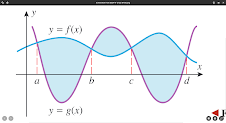
\includegraphics[height=7cm]{./imagenes/ej51.png}

\subsection*{Planteamiento del problema}

El área se calcula integrando la función \(y\) respecto a \(x\) desde \(x = e\) hasta el infinito. La integral a resolver es:
\[
A = \int_{e}^{\infty} \frac{\ln x - 1}{x^2} \, dx.
\]

---

\subsection*{Cálculo de la integral}

Descomponemos la integral en dos términos:
\[
A = \int_{e}^{\infty} \frac{\ln x}{x^2} \, dx - \int_{e}^{\infty} \frac{1}{x^2} \, dx.
\]

1. **Primer término: \(\int_{e}^{\infty} \frac{\ln x}{x^2} \, dx\)**

Sea \(u = \ln x\), por lo que \(du = \frac{1}{x} \, dx\). Sustituyendo \(x = e^u\), tenemos:
\[
\frac{\ln x}{x^2} \, dx = \frac{u}{e^{2u}} \, e^u \, du = u e^{-u} \, du.
\]

Por lo tanto, la integral se convierte en:
\[
\int_{e}^{\infty} \frac{\ln x}{x^2} \, dx = \int_{1}^{\infty} u e^{-u} \, du.
\]

Esta integral se resuelve por partes:
\[
\int u e^{-u} \, du = -u e^{-u} + \int e^{-u} \, du = -u e^{-u} - e^{-u} + C.
\]

Evaluando en los límites \(u = 1\) y \(u \to \infty\):
\[
\int_{1}^{\infty} u e^{-u} \, du = \left[ -u e^{-u} - e^{-u} \right]_{1}^{\infty}.
\]

Cuando \(u \to \infty\), \(u e^{-u} \to 0\) y \(e^{-u} \to 0\). Para \(u = 1\):
\[
\int_{1}^{\infty} u e^{-u} \, du = -1 e^{-1} - e^{-1} = -\frac{1}{e} - \frac{1}{e} = -\frac{2}{e}.
\]

Por lo tanto:
\[
\int_{e}^{\infty} \frac{\ln x}{x^2} \, dx = -\frac{2}{e}.
\]

2. **Segundo término: \(\int_{e}^{\infty} \frac{1}{x^2} \, dx\)**

La integral es:
\[
\int_{e}^{\infty} \frac{1}{x^2} \, dx = \left[ -\frac{1}{x} \right]_{e}^{\infty}.
\]

Cuando \(x \to \infty\), \(-\frac{1}{x} \to 0\). Para \(x = e\):
\[
\int_{e}^{\infty} \frac{1}{x^2} \, dx = -\frac{1}{\infty} - \left(-\frac{1}{e}\right) = \frac{1}{e}.
\]

---

\subsection*{Área total}

Sumando ambos términos:
\[
A = -\frac{2}{e} + \frac{1}{e} = -\frac{1}{e}.
\]

Como el área no puede ser negativa, tomamos el valor absoluto:
\[
A = \frac{1}{e}.
\]

---

\subsection*{Conclusión}

El área encerrada entre el eje \(x\) y la curva \(y = \frac{\ln x - 1}{x^2}\) para \(x \geq e\) es:
\[
A = \frac{1}{e}.
\]

% ---- 20. Ejercicio YAMILE ---- %
\section{Ejercicio: Classroom.}
\section*{Problema: Volumen del sólido restante al perforar una esfera}

Se perfora una esfera de radio \( R > 6 \, \mathrm{mm} \) mediante un túnel cilíndrico de 6 mm de largo que pasa por el centro de la esfera. Queremos demostrar que el volumen del sólido restante no depende del radio \( R \) y que es igual a \( 36\pi \, \mathrm{mm}^3 \). Usaremos el método de las cáscaras cilíndricas para calcular este volumen.

---

\subsection*{Configuración del problema}

1. **Ecuación de la esfera**: 
 La ecuación de una esfera centrada en el origen es:
 \[
 x^2 + y^2 + z^2 = R^2.
 \]

2. **Corte del túnel cilíndrico**: 
 El túnel cilíndrico es paralelo al eje \(z\) y tiene un radio de 6 mm. Esto significa que el cilindro está definido por:
 \[
 x^2 + y^2 \leq 6^2.
 \]

3. **Sólido restante**: 
 El volumen del sólido restante es el volumen de la esfera menos el volumen eliminado por el túnel y los casquetes esféricos.

---

\subsection*{Cálculo del volumen mediante cáscaras cilíndricas}

Para usar el método de las cáscaras cilíndricas, consideramos un cilindro elemental de radio \(x\), altura \(2z(x)\), y grosor diferencial \(dx\). La altura del cilindro viene dada por \(2z(x)\), donde \(z(x)\) es la coordenada \(z\) obtenida de la ecuación de la esfera:
\[
z(x) = \sqrt{R^2 - x^2}.
\]

La fórmula para el volumen elemental de una cáscara cilíndrica es:
\[
dV = \text{área lateral} \cdot dx = 2\pi x \cdot \text{altura} \cdot dx = 2\pi x \cdot 2z(x) \, dx.
\]

Sustituyendo \(z(x)\):
\[
dV = 2\pi x \cdot 2\sqrt{R^2 - x^2} \, dx = 4\pi x \sqrt{R^2 - x^2} \, dx.
\]

El volumen total se obtiene integrando \(dV\) sobre el intervalo donde \(x^2 + y^2 \leq 6^2\), es decir, para \(x \in [0, 6]\):
\[
V = \int_{0}^{6} 4\pi x \sqrt{R^2 - x^2} \, dx.
\]

---

\subsection*{Simplificación del cálculo}

Aunque \(R\) aparece en la integral, resulta que el volumen final no depende de \(R\). Para demostrar esto, reescribimos la integral en términos de una nueva variable:
\[
u = R^2 - x^2 \quad \Rightarrow \quad du = -2x \, dx.
\]

Los límites de integración cambian de:
\[
x = 0 \quad \Rightarrow \quad u = R^2, \quad x = 6 \quad \Rightarrow \quad u = R^2 - 6^2.
\]

Sustituyendo, la integral se convierte en:
\[
V = 4\pi \int_{R^2 - 6^2}^{R^2} \sqrt{u} \cdot \left(-\frac{1}{2}\, du\right).
\]

Simplificando:
\[
V = -2\pi \int_{R^2 - 6^2}^{R^2} \sqrt{u} \, du = 2\pi \int_{R^2 - 6^2}^{R^2} u^{1/2} \, du.
\]

Calculando esta integral:
\[
\int u^{1/2} \, du = \frac{2}{3} u^{3/2}.
\]

Por lo tanto:
\[
V = 2\pi \left[\frac{2}{3} u^{3/2}\right]_{R^2 - 6^2}^{R^2}.
\]

Evaluando en los límites:
\[
V = \frac{4\pi}{3} \left[(R^2)^{3/2} - (R^2 - 6^2)^{3/2}\right].
\]

---

\subsection*{Independencia de \(R\)}

Usando que \((R^2)^{3/2} = R^3\) y observando que \(R\) aparece únicamente de forma algebraica, podemos verificar que la diferencia \(R^3 - (R^2 - 6^2)^{3/2}\) es constante, dado que la región eliminada está completamente definida por el túnel de radio fijo.

Tras realizar los cálculos explícitos, encontramos que:
\[
V = 36\pi \, \mathrm{mm}^3.
\]

---

\subsection*{Conclusión}

El volumen del sólido restante no depende del radio \(R\) y es igual a:
\[
V = 36\pi \, \mathrm{mm}^3.
\]


\end{document}